\documentclass[tikz,border=10pt]{standalone}
\usepackage{tikz}
\usetikzlibrary{arrows.meta, calc, decorations.pathmorphing, decorations.markings, angles, quotes}

\begin{document}

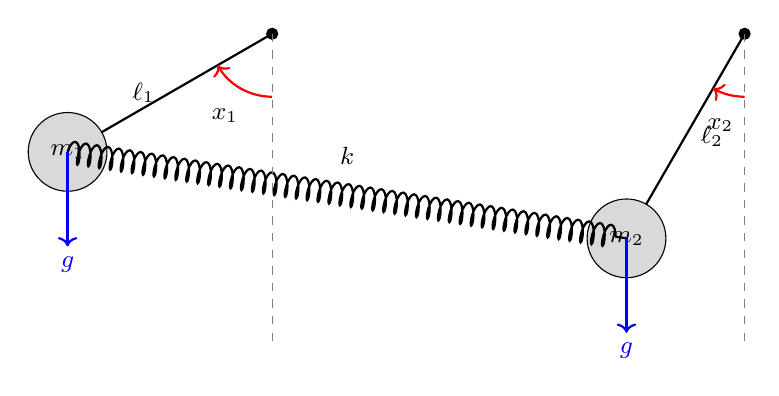
\begin{tikzpicture}[
  mass/.style = {circle, draw, fill=gray!30, minimum size=1cm},
  string/.style = {thick},
  spring/.style = {thick, decorate, decoration={aspect=0.3, segment length=4pt, amplitude=4pt, coil}},
  force/.style = {->, thick, blue},
  anglemark/.style = {draw, ->, thick, red},
  every node/.style = {font=\small}
]

% Parameters
\def\Lone{3}
\def\Ltwo{3}
\def\thetaone{30}
\def\thetatwo{60}

% Coordinates
\coordinate (pivot1) at (-3, 0);
\coordinate (pivot2) at (3, 0);
\coordinate (m1) at ($(pivot1) + (\thetaone:-\Lone)$);
\coordinate (m2) at ($(pivot2) + (\thetatwo:-\Ltwo)$);

% Pendulum arms
\draw[string] (pivot1) -- (m1);
\draw[string] (pivot2) -- (m2);

% Masses and pivots
\filldraw[black] (pivot1) circle (2pt);
\filldraw[black] (pivot2) circle (2pt);
\node[mass] at (m1) {$m_1$};
\node[mass] at (m2) {$m_2$};

% Spring between masses
\draw[spring] (m1) -- (m2);
\node at ($(m1)!0.5!(m2) + (0,0.5)$) {$k$};

% Gravity vectors
\draw[force] (m1) -- ++(0,-1.2) node[below] {$g$};
\draw[force] (m2) -- ++(0,-1.2) node[below] {$g$};

% Length labels
\path (pivot1) -- node[midway, left=2pt] {$\ell_1$} (m1);
\path (pivot2) -- node[midway, right=2pt] {$\ell_2$} (m2);

% Vertical dashed lines
\draw[dashed, gray] (pivot1) -- ++(270:\Lone+1);
\draw[dashed, gray] (pivot2) -- ++(270:\Ltwo+1);

% Angle arcs
\draw[anglemark] (pivot1) ++(270:0.8) arc[start angle=270, end angle={270 - \thetatwo}, radius=0.8];
\node at ($(pivot1)+({270 - 0.5*\thetatwo}:1.2)$) {$x_1$};

\draw[anglemark] (pivot2) ++(270:0.8) arc[start angle=270, end angle={270 - \thetaone}, radius=0.8];
\node at ($(pivot2)+({270 - 0.5*\thetaone}:1.2)$) {$x_2$};

\end{tikzpicture}

\end{document}
